% 
% topic Template for ME3023 - Measurements in Mechanincal Systems - Tennessee Technological University
%
% Spring 2020 - Summer 2020
% Tristan Hill, May 31, 2020
% Module 2 - To Err is Human 
% Topic 4 - Accuracy and Precesion
%

\documentclass{beamer}                         % for presentation (has nav buttons at bottom)
%\documentclass[handout]{beamer}  % for handout 
\usepackage{beamerthemesplit}
\usepackage{amsmath}
\usepackage{listings}
\usepackage{multicol}
\usepackage{framed}

\beamertemplateballitem

\definecolor{TTUpurple}{rgb}{0.3098, 0.1607, 0.5176} % TTU Purple (primary)
\definecolor{TTUgold}{rgb}{1.0000, 0.8666, 0.0000} % TTU Gold (primary)

\setbeamercolor{palette primary}{bg=TTUpurple,fg=TTUgold}
\setbeamercolor{palette secondary}{bg=black,fg=TTUgold}
\setbeamercolor{palette tertiary}{bg=black,fg=TTUpurple}
\setbeamercolor{palette quaternary}{bg=TTUgold,fg=black}
\setbeamercolor{structure}{fg=TTUpurple} % itemize, enumerate, etc
\setbeamercolor{section in toc}{fg=TTUpurple} % TOC sections

% custom colors 
\definecolor{mygray}{rgb}{.6, .6, .6}
\definecolor{mypurple}{rgb}{0.6,0.1961,0.8}
\definecolor{mybrown}{rgb}{0.5451,0.2706,0.0745}
\definecolor{mygreen}{rgb}{0, .39, 0}
\definecolor{mypink}{rgb}{0.9960, 0, 0.9960}

% color commands
\newcommand{\R}{\color{red}}
\newcommand{\B}{\color{blue}}
\newcommand{\BR}{\color{mybrown}}
\newcommand{\K}{\color{black}}
\newcommand{\G}{\color{mygreen}}
\newcommand{\PR}{\color{mypurple}}

\newcommand{\PN}{\color{mypink}}
%\usefonttheme{professionalfonts}

\newcommand{\Lagr}{\mathcal{L}} % lagrangian

\newcommand{\vspccc}{\vspace{6mm}\\} % large vertical space
\newcommand{\vspcc}{\vspace{4mm}\\}   % medium vertical space
\newcommand{\vspc}{\vspace{2mm}\\}     % small vertical space

\newcommand{\hspcccc}{\hspace{10mm}} % large horizontal space
\newcommand{\hspccc}{\hspace{6mm}} % large horizontal space
\newcommand{\hspcc}{\hspace{4mm}}   % medium horizontal space
\newcommand{\hspc}{\hspace{2mm}}     % small horizontal space


\author{ME3023 - Measurements in Mechanical Systems} % original formatting from Mike Renfro, September 21, 2004

\newcommand{\MNUM}{2\hspace{2mm}} % Module number
\newcommand{\TNUM}{4\hspace{2mm}} % Topic number 
\newcommand{\moduletitle}{To Err is Human }
\newcommand{\topictitle}{Accuracy and Error } 

\title{Module \MNUM - \moduletitle}

\date{June 02, 2020}

\begin{document}

\lstset{language=MATLAB,basicstyle=\ttfamily\small,showstringspaces=false}

\frame{\titlepage \center\begin{framed}\Large \textbf{Topic \TNUM - \topictitle}\end{framed} \vspace{5mm}}

% Section 0: Outline

\frame{

\large \textbf{Topic \TNUM - \topictitle} \vspace{3mm}\\

\begin{itemize}
	\item Thought Experiment \vspc % Section 1
	\item Accuracy and Error \vspc% Section 2
	\item Estimating Error\vspc% Section 3
	\item Random and Systematic Errors \vspc%Section 4
	\item Dart Board Example \vspc%Section 5
\end{itemize}

}

% Section 2
\section{Thought Experiment}

\frame{
\frametitle{Thought Experiment}

{\bf Thought Experiment}: Look around the room and choose an object. It can be anything. Ask yourself the following questions. \vspc
\begin{itemize}
\item What is the {\bf\G true} length of the object? \vspc
\item How can you find the {\bf\G true} value? Can you measure it? \vspc
\item ...
\end{itemize}

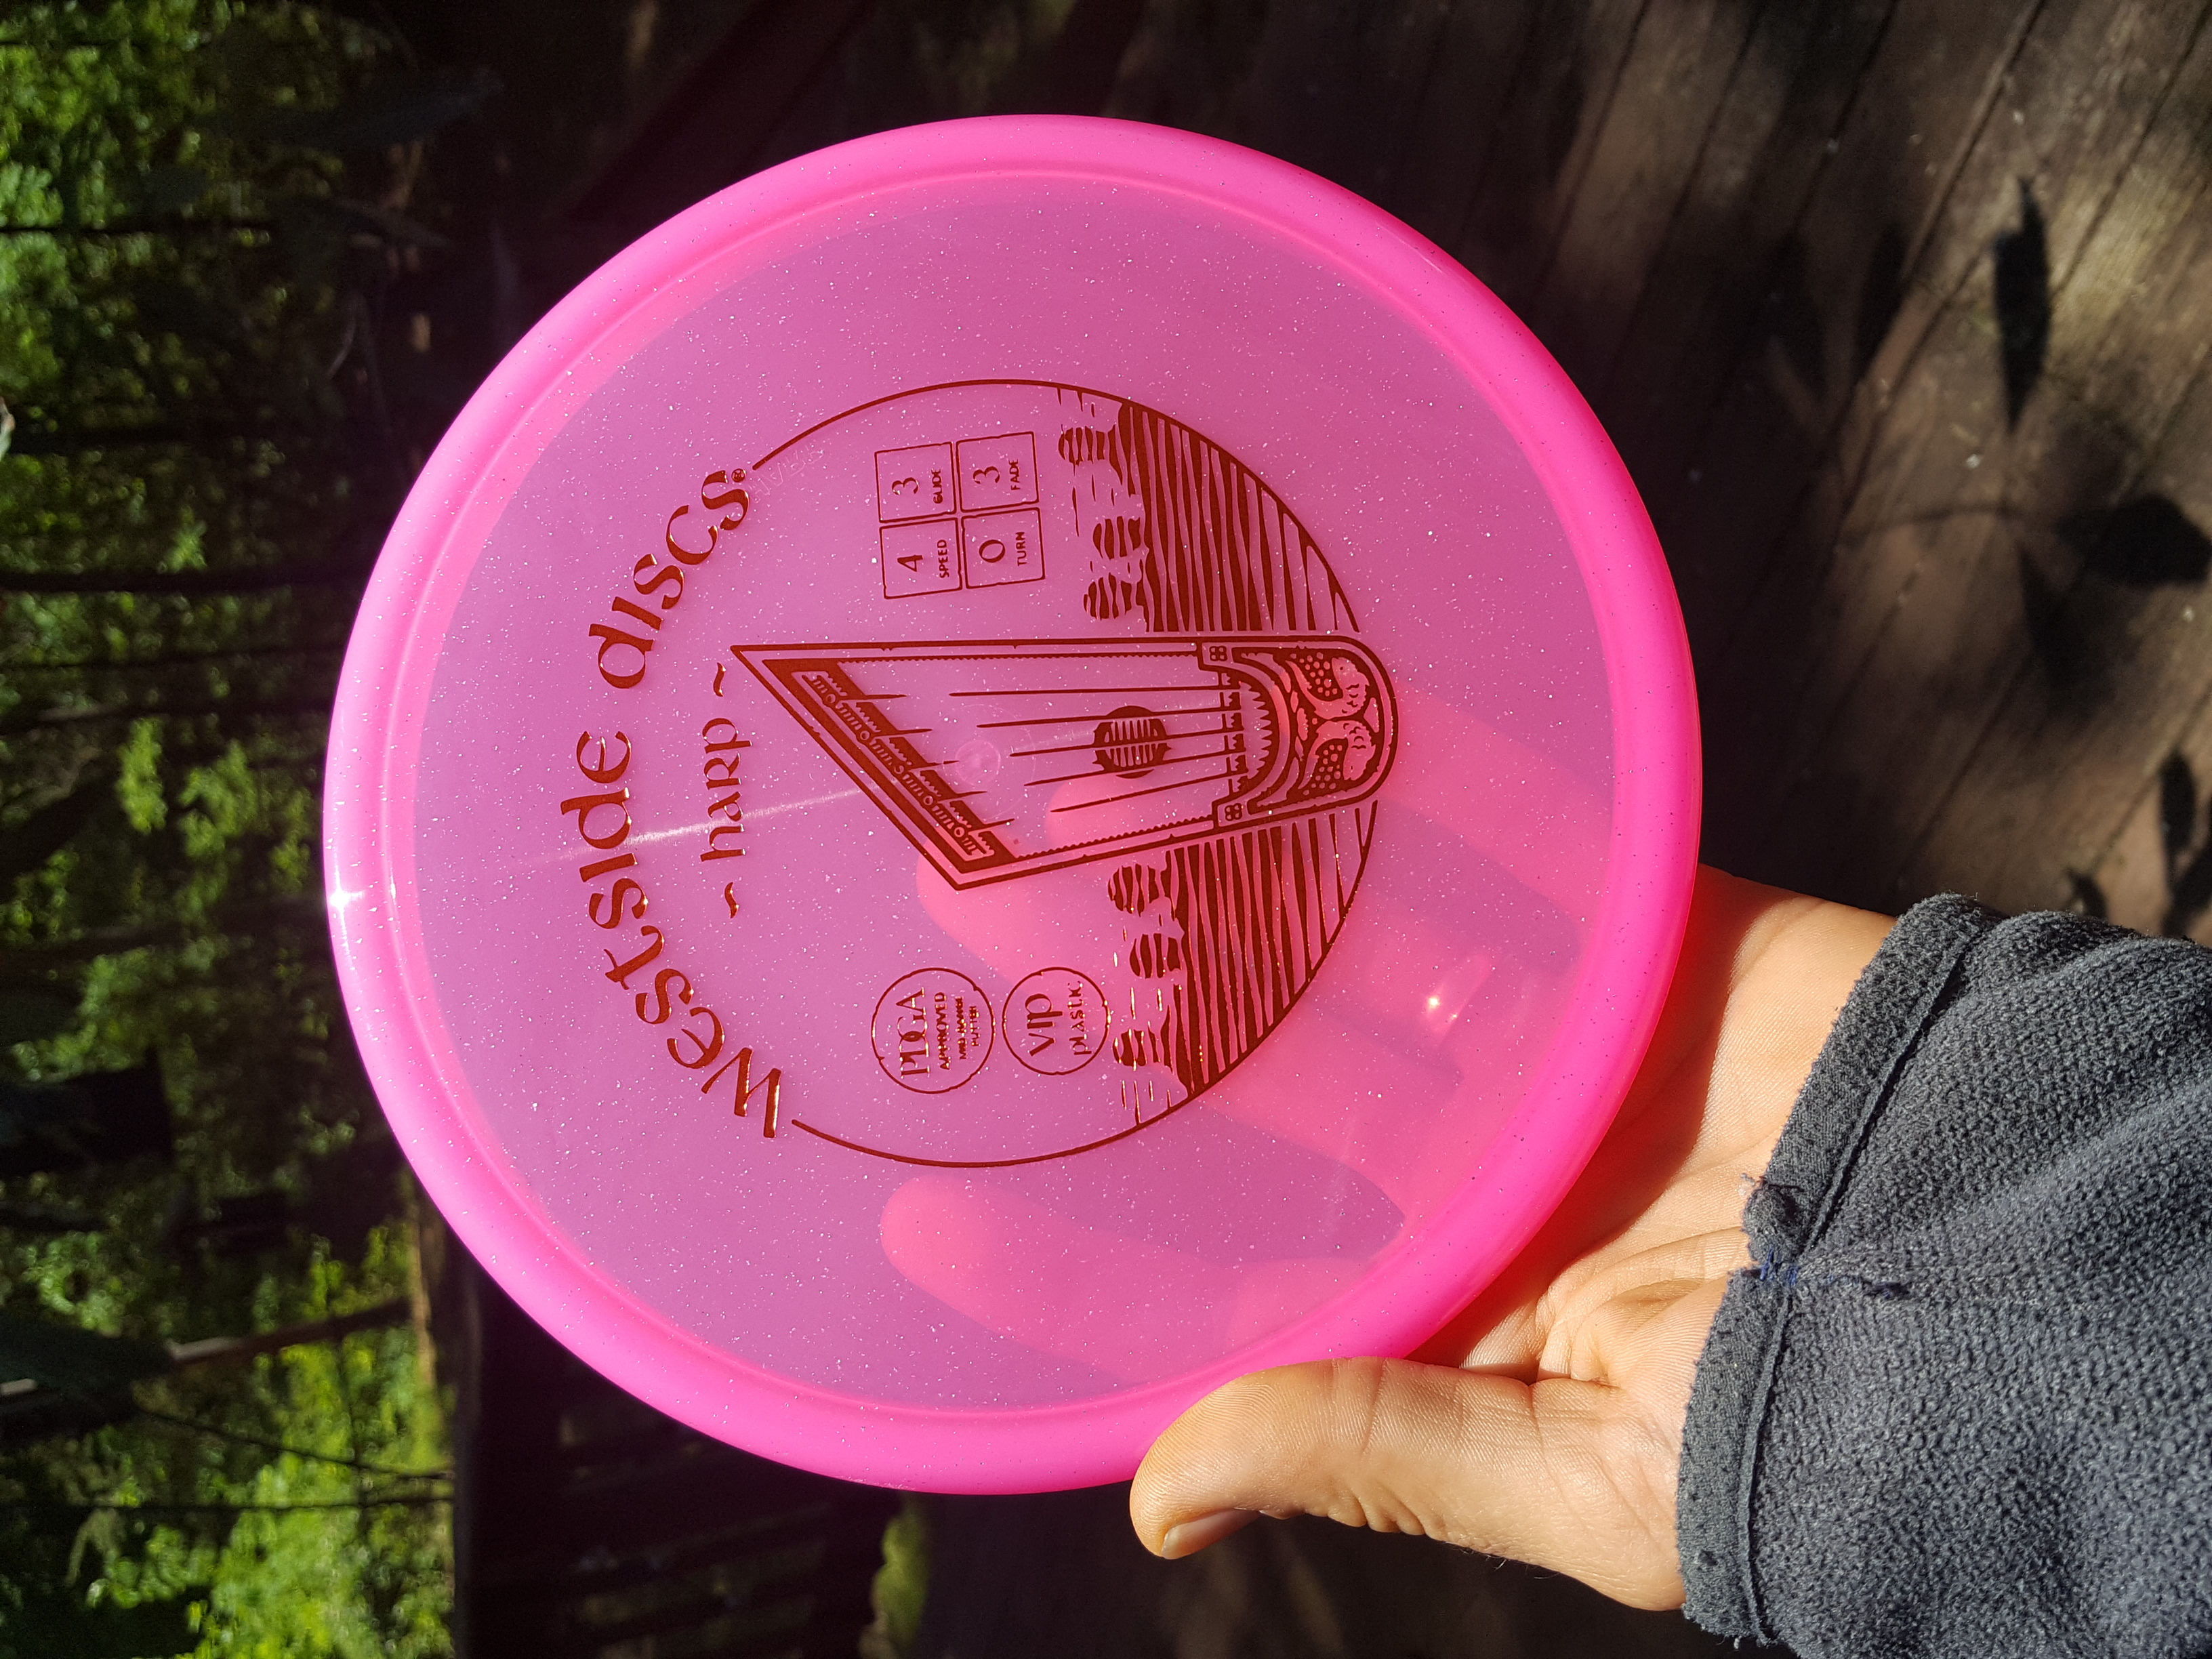
\includegraphics[scale=.025,angle=-90,origin=c]{vip_harp.jpg}
{\tiny Image: T.Hill}
}

% Section 1
\section{True and Measured Value}

\frame{
\frametitle{True and Measured Value}

The exact value of a variable is called the {\G true value}. The value of the variables as indicated by a
measurement system is called the {\B measured value}. The {\PR accuracy} of a measurement refers to the
closeness of agreement between the measured value and the true value. But the {\G true value} is rarely
known {\it exactly}, and various influences, called {\R errors}, have an effect on both of these values. So the
concept of the {\PR accuracy} of a measurement is a {\it qualitative} one. \vspcc

\begin{framed}\scalebox{1}{$\hspace{10mm}{\R error} = {\B measured\hspace{1mm}value} - {\G true\hspace{1mm}value} $}\end{framed}

\vspace{0mm}
{\tiny Text: Theory and Design of Mech. Meas.}
}

% Section 3
\section{Estimating Error}

\frame{
\frametitle{Estimating Error}

The {\bf \G true value} can be estimated but cannot not be known  {\it exactly}. In practice a {\BR reference} value is used in place of the true value. We will discuss this again the the {\it Calibration Module}.


\begin{framed}\scalebox{1}{$\hspace{20mm} {\PR accuracy} =  \frac{|{\R error}|}{{\BR reference\hspace{1mm}value}}\times 100 $}\end{framed}

An estimate of error based using this value is sometimes referred to as {\B relative accuracy}. \vspc


%{\tiny Text: Theory and Design of Mech. Meas.}
}
% Section 3
\section{Random and Systematic Errors}

\frame{
\frametitle{Random and Systematic Errors}

``Errors are effects that cause a  measured value to differ from its true value. {\PN Random} error causes a
{\PN random} variation in measured values found during repeated measurements of a variable. {\PR Systematic}
error causes an offset between the mean value of the data set and its true value. Both {\PN random} and
{\PR systematic} errors affect a system’s accuracy.''

\vspace{10mm}
{\tiny Text: Theory and Design of Mech. Meas.}
}

% Section 4
\section{Dart Board Example}

\frame{
\frametitle{Dart Board Example}

``The concept of accuracy and the effects of {\PR systematic} and {\PN random} errors in instruments
and measurement systems can be illustrated by the throw of darts.''

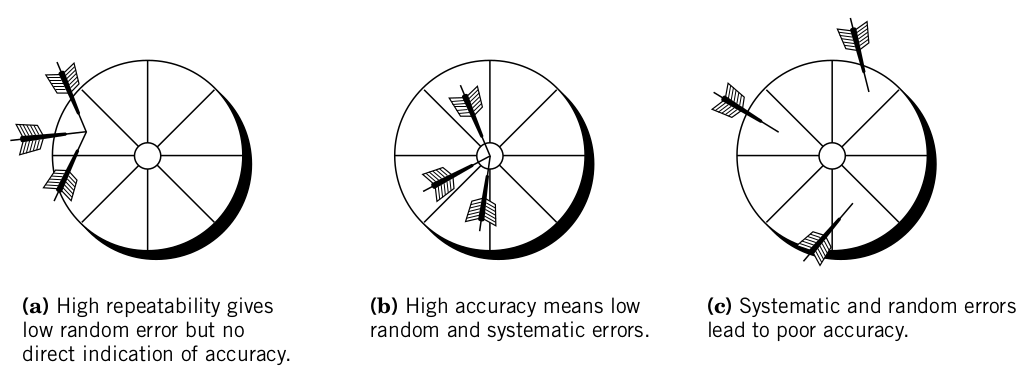
\includegraphics[scale=.20]{dart_throw.png}

``The ability of a measurement system to indicate the same value on repeated but independent
application of the same input provides a measure of the instrument {\B repeatability}.''

{\tiny Text, Image: Theory and Design of Mech. Meas.}
}


\end{document}





